
\documentclass[aspectratio=169]{beamer}

%\setbeameroption{hide notes}
%\setbeameroption{show notes}
%\setbeameroption{show only notes}

  % Copyright (C) 2012 - EDF R&D - Michael Baudin

% To highlight source code
\usepackage{listings}
\definecolor{darkgreen}{rgb}{0,0.5,0}
\definecolor{violet}{rgb}{0.5,0,1}

\usepackage{lmodern}% http://ctan.org/pkg/lm

\usetheme{Montpellier}
\setbeamertemplate{navigation symbols}{} % Remove navigation
\useoutertheme{infolines}

\usepackage[utf8]{inputenc}
\usepackage[T1]{fontenc}

%\usepackage[french]{babel}
%\uselanguage{French}
%\languagepath{French}

\def\bx{{\bf x}}
\def\RR{\mathbb{R}}

\newcommand{\pyvar}[1]{\texttt{#1}}

\def \ot {OpenTURNS}

\usepackage{adjustbox}
\usepackage[normalem]{ulem}

\title[OpenTURNS]{OpenTURNS release highlights}

\author[OpenTURNS et al.]{J. Schueller (Phimeca)}

% \institute[Airbus-EDF-IMACS-ONERA-Phimeca]{
% \inst{1} Airbus
% \inst{2} EDF R\&D. 6, quai Watier, 78401, Chatou Cedex - France, michael.baudin@edf.fr \and %
% \inst{3} IMACS
% \inst{4} ONERA
% \inst{5} Phimeca Engineering. 18/20 boulevard de Reuilly, 75012 Paris - France, schueller@phimeca.com
% }

\date[]{User Day \#17, June 14th 2024, EDF Lab}
%%%%%%%%%%%%%%%%%%%%%%%%%%%%%%%%%%%%%%%%%%%%%%%%%%%%%%%%%%%%%%%%%%%%%%%%%%%%%

  \begin{document}

%%%%%%%%%%%%%%%%%%%%%%%%%%%%%%%%%%%%%%%%%%%%%%%%%%%%%%%%%%%%%%%%%%%%%%%%%%%%%

  \begin{frame}
  \titlepage

  \begin{columns}
  \begin{column}[t]{0.05\textwidth}
        \end{column}
  
    \column{0.10\textwidth}
  \begin{center}

\includegraphics[height=0.04\textheight]{figures/airbus-logo-3d-blue.png}
\end{center}

    \column{0.05\textwidth}
  \begin{center}

\includegraphics[height=0.09\textheight]{figures/logo-edf.jpg}
\end{center}

     \column{0.05\textwidth}
  \begin{center}

\includegraphics[height=0.09\textheight]{figures/imacs-logo.jpg}
\end{center}

    \column{0.10\textwidth}
  \begin{center}

\includegraphics[height=0.05\textheight]{figures/onera-logo.png}
\end{center}

    \column{0.15\textwidth}
  \begin{center}

\includegraphics[height=0.08\textheight]{figures/logo-phimeca.png}
\end{center}

\column{0.01\textwidth}

  \end{columns}

  \end{frame}

\begin{frame}
\frametitle{Overview}

New features since last year in releases:

\begin{itemize}
\item v1.22: fall 2023
\item v1.23: spring 2024
\end{itemize}

\end{frame}
  
%%%%%%%%%%%%%%%%%%%%%%%%%%%%%%%%%%%%%%%%%%%%%%%%%%%%%%%%%%%%%%%%%%%%%%%%%%%%%

% \begin{frame}
% \frametitle{Contents}
% % \tableofcontents
% \end{frame}

%%%%%%%%%%%%%%%%%%%%%%%%%%%%%%%%%%%%%%%%%%%%%%%%%%%%%%%%%%%%%%%%%%%%%%%%%%%%%

\begin{frame}{UniformOrderStatistics}

\begin{itemize}
\item Joint distribution of the order statistics
\end{itemize}

\begin{figure}[!htb]
\minipage{0.5\textwidth}
  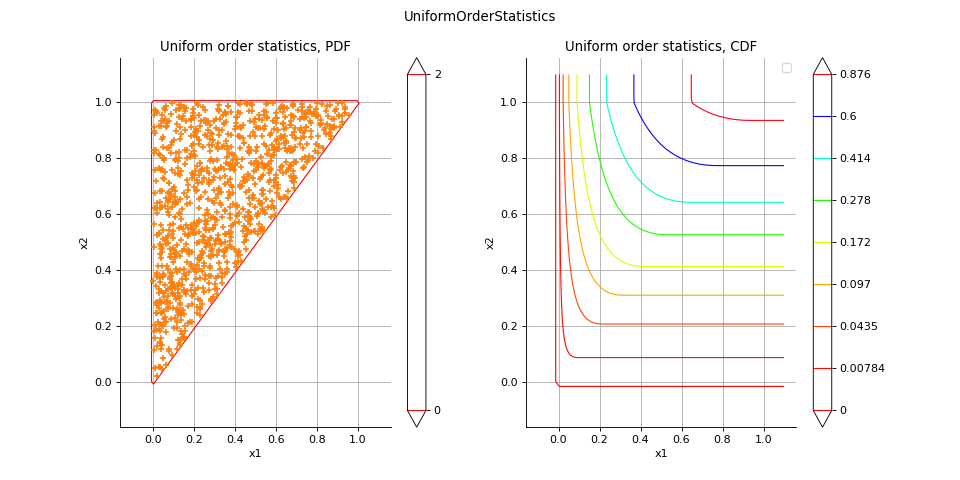
\includegraphics[width=1.3\textwidth]{figures/UniformOrderStatistics}
\endminipage\hfill
\end{figure}
\end{frame}

%%%%%%%%%%%%%%%%%%%%%%%%%%%%%%%%%%%%%%%%%%%%%%%%%%%%%%%%%%%%%%%%%%%%%%%%%%%%%

% \section{Truncated distribution over a mesh}

\begin{frame}{Truncated distribution over a mesh}
% \begin{block}
\begin{itemize}
\item Generalization of UniformOverMesh
\item Sampling following any distribution in any closed set delimited by a generic mesh, any dimension
% \item Sampling of simplices weighted by volume, then uniform sampling inside simplex
% \item CDF is obtained by integration at mesh bounds
% \item Efficient implementation, low-level primitives for tetras, etc ...
\end{itemize}
% \end{block}
\begin{figure}
   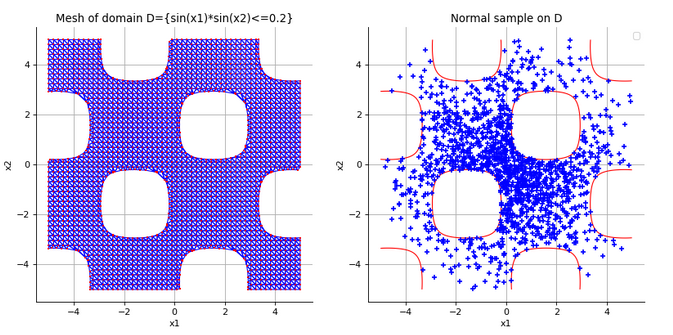
\includegraphics[width=0.6\textwidth]{figures/TruncatedOverMesh}
\end{figure}
\end{frame}

%%%%%%%%%%%%%%%%%%%%%%%%%%%%%%%%%%%%%%%%%%%%%%%%%%%%%%%%%%%%%%%%%%%%%%%%%%%%%

\begin{frame}{Other new distributions}
% \begin{block}
\begin{itemize}
\item StudentCopula
\item StudentCopulaFactory
\item SmoothedUniformFactory
\item New GEV/GPD estimators
% \item CDF is obtained by integration at mesh bounds
% \item Efficient implementation, low-level primitives for tetras, etc ...
\end{itemize}
% \end{block}
% \begin{figure}
%    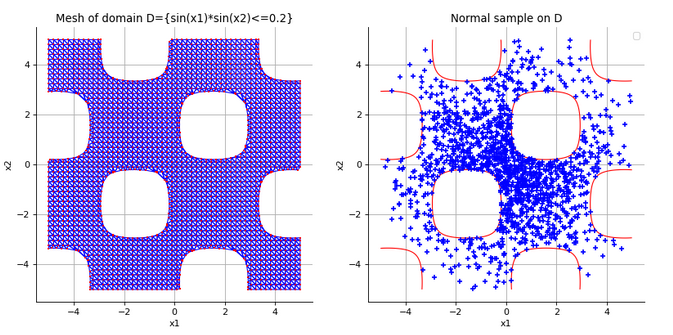
\includegraphics[width=0.6\textwidth]{figures/TruncatedOverMesh}
% \end{figure}
\end{frame}


%%%%%%%%%%%%%%%%%%%%%%%%%%%%%%%%%%%%%%%%%%%%%%%%%%%%%%%%%%%%%%%%%%%%%%%%%%%%%

\begin{frame}{Latent variable model}

\begin{itemize}
\item Covariance model allowing to compute the covariance between different unordered values (or levels) of a categorical variable
\end{itemize}

% \begin{figure}
%    \includegraphics[width=0.5\textwidth]{figures/sphx_glr_plot_crossentropy_003}
%    \includegraphics[width=0.35\textwidth]{figures/crossads}
% \end{figure}

\end{frame}

%%%%%%%%%%%%%%%%%%%%%%%%%%%%%%%%%%%%%%%%%%%%%%%%%%%%%%%%%%%%%%%%%%%%%%%%%%%%%

\begin{frame}
\frametitle{New field metamodeling capabilities}
\begin{itemize}
\item Vector to field metamodeling and sensitivity using KL + chaos
% \item Efficient trace computation in HSICVStat instead of full products
% \item Cache input covariance matrix discretization
% \item Use STL primitives like std::accumulate
\end{itemize}

\end{frame}


%%%%%%%%%%%%%%%%%%%%%%%%%%%%%%%%%%%%%%%%%%%%%%%%%%%%%%%%%%%%%%%%%%%%%%%%%%%%%

\begin{frame}
\frametitle{Rank-based Sobol' indices}
\begin{itemize}
\item Data-driven (no need for dedicated design of experiments)
\item RankSobolSensitivityAlgorithm
% \item Efficient trace computation in HSICVStat instead of full products
% \item Cache input covariance matrix discretization
% \item Use STL primitives like std::accumulate
\end{itemize}

\end{frame}

%%%%%%%%%%%%%%%%%%%%%%%%%%%%%%%%%%%%%%%%%%%%%%%%%%%%%%%%%%%%%%%%%%%%%%%%%%%%%

\begin{frame}
\frametitle{Documentation improvements}
\begin{itemize}
\item Lots of new examples: chaos, cv, regression, MLE, functions, integration, enumerate, ...
\item New usecases: fire satellite, wing weight, Linthurst/Coles datasets
\end{itemize}

\begin{center}

\includegraphics[width=0.3\textwidth]{figures/stiffened_panel_simulation}
\end{center}

\begin{itemize}
\item Example minigalleries linking to relevant examples
\item Lot of time invested in the improvement of the documentation
\end{itemize}
\end{frame}

%%%%%%%%%%%%%%%%%%%%%%%%%%%%%%%%%%%%%%%%%%%%%%%%%%%%%%%%%%%%%%%%%%%%%%%%%%%%%

\begin{frame}
\frametitle{Other improvements}
\begin{itemize}
\item Multidimensional integration using cuba library (CubaIntegration)
\item New class for integration from an existing design of experiment (ExperimentIntegration)
\item Boundary extraction based on external faces simplices (BoundaryMesher)
\item Faster marginal PDF extraction (speedup for BayesDistribution)
\item Faster KDTree implementation using nanoflann library
\item Faster TruncatedDistribution with n-d CDF inversion
\end{itemize}

\vspace{6pt}

\begin{center}
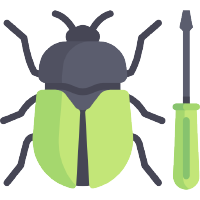
\includegraphics[width=0.15\textwidth]{figures/bugfix}
\end{center}

\end{frame}

%%%%%%%%%%%%%%%%%%%%%%%%%%%%%%%%%%%%%%%%%%%%%%%%%%%%%%%%%%%%%%%%%%%%%%%%%%%

\begin{frame}
\frametitle{Packaging 1/2}
\begin{block}{Python channels}
\begin{itemize}
\item Pip (and uv), Conda
\item Versions: 3.8-3.12
\item OS: Windows, Linux, MacOS
\item Architectures: x86\_64, arm64 (MacOS-only)
\end{itemize}
\end{block}

\begin{figure}
   
\includegraphics[width=0.3\textwidth]{figures/PyPI_logo}
   
\includegraphics[width=0.3\textwidth]{figures/Conda_logo.svg}
\end{figure}

\end{frame}

\begin{frame}
\frametitle{Packaging 2/2}
\begin{block}{Supported Linux distributions}
\begin{itemize}
\item Ubuntu 22/24
\item Debian 11/12
\item Fedora 39/40
\item CentOS 8
\item OpenSUSE 15.5
\item Mageia 8
\item ArchLinux
\end{itemize}

... and FreeBSD

\end{block}


\begin{center}

\includegraphics[width=0.05\textwidth]{figures/debian-openlogo-100}

\includegraphics[width=0.08\textwidth]{figures/ubuntu}

\includegraphics[width=0.08\textwidth]{figures/Fedora-Logo}

\includegraphics[width=0.08\textwidth]{figures/centos-logo}

\includegraphics[width=0.08\textwidth]{figures/opensuse-logo}

\includegraphics[width=0.15\textwidth]{figures/200px-Logo_mageia_official}

\includegraphics[width=0.15\textwidth]{figures/archlinux-logo}

\includegraphics[width=0.15\textwidth]{figures/FREEBSD_Logo_Horiz_Pos_RGB}
\end{center}

\end{frame}

%%%%%%%%%%%%%%%%%%%%%%%%%%%%%%%%%%%%%%%%%%%%%%%%%%%%%%%%%%%%%%%%%%%%%%%%%%%%%

\begin{frame}
\frametitle{END}

Thank you for your attention!

Any questions?

\begin{center}
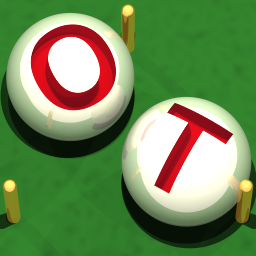
\includegraphics[width=0.2\textwidth]{figures/logo-ot-small}
\end{center}

\end{frame}

% %%%%%%%%%%%%%%%%%%%%%%%%%%%%%%%%%%%%%%%%%%%%%%%%%%%%%%%%%%%%%%%%%%%%%%%%%%%%%
% 
% \section{Bibliography}
% 
% \begin{frame}
% \frametitle{Bibliography}
% 
% \begin{itemize}
% \item Airbus, EDF, ONERA, Phimeca Engineering, IMACS.
% OpenTURNS, a scientific library usable as a Python module dedicated to the treatment of uncertainties, 
% \url{www.openturns.org}.
% \item Airbus, EDF, Phimeca Engineering, IMACS. Documentation of OpenTURNS, version 1.9. 
% \url{http://openturns.github.io/openturns/1.9/contents.html}
% \item  Michaël Baudin, Anne Dutfoy, Bertrand Iooss, and Anne-Laure Popelin. 
% OpenTURNS: An Industrial Software for Uncertainty Quantification in Simulation, 
% Handbook of Uncertainty Quantification, 
% pages 1-38. Springer International Publishing, 2016
% \end{itemize}
% 
% \end{frame}

\end{document}
